\documentclass[10pt]{article}

% import a set of useful packages for math
\usepackage{amsmath, amssymb,amsthm,xspace}

% for importing images
\usepackage{graphicx}
\usepackage{xcolor}

% for algorithm environments
\usepackage{algorithm}     % creates the float "Algorithm 1: My Algorithm"
\usepackage{algorithmic}   % for the algorithm itself, e.g. "for x = 1 to n..."
\usepackage{braket}
\usepackage{tikz}

%%%% import any other packages here
\usepackage{fancyhdr}
\usepackage{listings}
\usepackage{indentfirst}
\usepackage{hyperref}
\usepackage{perpage}
\usepackage{mathtools}
% \MakePerPage{footnote}

\newtheorem{lemma}{Lemma}
\newtheorem{theorem}{Theorem}
\newtheorem{definition}{Definition}
\newtheorem{corollary}{Corollary}
\newtheorem{conjecture}{Conjecture}

\pagestyle{fancy}
% \rhead{KORDONOWY}

\begin{document}

\title{Classical + Quantum Algorithms for Local Max-Cut}
\date{}
\maketitle

\section*{Conjectures}


\section*{Happiness}
Let $G = (V,E)$ be a graph of order $n \geq 3$ with degree 2 (a ring). A  \emph{cut} is a bitstring $c=(c_0 \dots c_{2^n - 1})$. A $v \in V$ is \emph{happy for cut c} when 

\begin{equation}
|\{u \in V\setminus \{v\} : c_u \neq c_v \}| \geq |\{u \in V\setminus \{v\} : c_u = c_v \}|
\end{equation}

\noindent ie when there are at least a many of $v$'s neighbors on the opposite side of the cut as on the same side. 

\begin{definition}
    For $d=2$, define the \underline{happiness function} $h : \mathbb{Z}_5 \times \{0,1\}^5$ by
\begin{equation}
    h(v,\mathbf{c}) =\ !(c_{v-1} = c_v = c_{v+1})
\end{equation}
\end{definition}
Should be full $n$ but need to determine how to get a vertex's (second) neighborhood from the bitstring $\textbf{c}$

\section*{Hamiltonian}
The goal is to construct a Hermitian operator $H: \{0,1\}^n \rightarrow \mathbb{N}$ that represents how many happy vertices are contained in $G$ for each possible cut. That is, $\bra{i}H\ket{i}$ is equal to the amount of happy vertices there are in $G$ for cut $i$. 
\begin{definition}
For $\mathbf{c} \in \{0,1\}^n$,
\begin{equation}
    H(\mathbf{c}) = \sum_{i \in V} h(i, \mathbf{c})
\end{equation}
\end{definition}

\subsection*{Full Graph Solution}
Given access to the full graph $G = (V,E)$, then we can naively construct $H$ by iterating over the possible cuts and counting how many $v \in V$ are happy.

\subsection*{Second Neighborhood Approach}
We construct $H$ by decomposing into $H_i$ for all $i \in V$ where $H_i$ counts the number of happy vertices in the neighborhood of $i$. To determine if $i - 1$ and $i+1$ are happy, we only need to know the second neighborhood of $i$. Therefore we are only interested in the 5 slots of the cut that correspond to $v's$ second neighbors.

We define $H_i : \{0,1\}^5 \rightarrow \mathbb{N}$ as
\begin{equation}
    H_i(\mathbf{c}) = h(i-1, \mathbf{c}) + h(i,\mathbf{c}) + h(i+1, \mathbf{c})
\end{equation}


\begin{theorem}
    $H = \frac{1}{3}\sum_{i \in V} H_i$.
\end{theorem}

\noindent Proof: For any cut $c \in \{0,1\}^n$, we have
\begin{align*}
    \bra{c}\frac{1}{3}\sum_{i \in V} H_i \ket{c} &= \frac{1}{3}\sum_{i \in V}\bra{c} H_i \ket{c} &\text{Linearity of expectation} \\
    & = \frac{1}{3}\sum_{i \in V}[h(i-1, \mathbf{c}) + h(i,\mathbf{c}) + h(i+1, \mathbf{c})] &\text{(4)} \\
    &= \sum_{i \in V} h(i, \mathbf{c}) &\text{Triple count each $h(j,\textbf{c})$ above} \\
    &= H &\text{(3)}
\end{align*}
\qed

\subsection*{Permutations}
Let $\sigma_n : \{0,1\}^n \rightarrow \{0,1\}^n$ be the finite left shift operator:
\begin{align}
    \sigma_n(c_0, c_1, \dots, c_{n-1}) = (c_1, c_2,\dots, c_{n-1}, c_0)
\end{align}

\begin{lemma}
    $\sigma_n$ is a permutation on $\{0,1\}^n$. 
\end{lemma}

\noindent Proof: For any $y = (y_0,\dots, y_{n-1}) \in \{0,1\}^n$, we have $\sigma_n(y_{n-1},y_0\dots, y_{n-2}) = y$. Now let $x =(x_0,\dots, x_{n-1}), y =(y_0,\dots, y_{n-1})\in \{0,1\}^n$ such that \\$\sigma_n(x) = \sigma_n(y)$. Then $(x_1,\dots, x_{n-1}, x_0) = (y_1,\dots, y_{n-1}, y_0)$ which is true iff $x_i = y_i$ for all $i$ and thus $x = y$. Therefore $\sigma_n$ is a bijection and since its domain and codomain are equal, it is a permutation. \qed

\begin{lemma}
All cycles of $\sigma_n$ are of order $n$ (except for the all 0s and all 1s strings in which $\sigma_n$ acts as the identity).
\end{lemma}
\noindent Proof: Let $x = (x_0, \dots, x_{n-1}) \in \{0,1\}^n$. Then $\sigma(x) = (x_1, \dots, x_{n-1}, x_0)$, $\sigma^2(x) = (x_2, \dots, x_0, x_1)$, etc, to $\sigma^{n-1}(x) = (x_{n-1}, x_0, \dots, x_{n-2}) \neq x$. Then
\begin{align*}
    \sigma^n(x) &= \sigma(\sigma^{n-1})(x) \\
    &= \sigma(x_{n-1}, x_0, \dots, x_{n-2}) \\
    &= (x_0, \dots, x_{n-1}) \\
    &=  x
\end{align*}

Lastly consider the string $(x, \dots, x)$ where $x \in \{0,1\}$. Then \\$\sigma(x, \dots, x) = (x, \dots, x)$.\qed

Next define the following function on $\mathbb{Z}_{2^n}$:

\begin{equation}
    \pi_n(i) = \begin{cases}
        2i &\text{if $0 \leq i < 2^{n-1}$} \\
        2i + 1 &\text{if $2^{n-1} \leq i < 2^n$}
    \end{cases}
\end{equation}

Remember that $i \in \mathbb{Z}_{2^n}$ so if $2i + 1 > 2^n$ then we need to subtract $2^n$ it.

\begin{lemma}
    $\pi_n$ is a permutation of $\mathbb{Z}_{2^n}$.
\end{lemma}
\noindent Proof: Let $y \in \mathbb{Z}_{2^n}$. If $y$ is even, then it can be written as $y = 2m$ for some $m \in \mathbb{Z}_{2^{n-1}}$. Then $\pi_n(m) = y$. If $y$ is odd, then it can be written as $y = 2m + 1$ for some $m \in \mathbb{Z}_{2^n}$. If $2^{n-1} \leq m < 2^n$, then $\pi_n(m) = y$. Otherwise, consider what happens if we replace $m$ with $m' = m + 2^{n-1}$:
\begin{align*}
    2m' + 1 = 2(m + 2^{n-1}) + 1 = 2m + 2^n + 1 \equiv 2m + 1 \mod 2^n
\end{align*}
And so $\pi_n(m') = y$ where $2^{n-1} \leq m' < 2^n$. Therefore $\pi_n$ is a bijection and since its domain and codomain are equal, it is a permutation. \qed

Now consider the function $f:\{0,1\}^n \rightarrow \mathbb{Z}_{2^n}$ given by 
\begin{equation}
    f_n((x_0, \dots, x_{n-1})) = \sum_{i=0}^{n-1} x_i \cdot 2^i
\end{equation}
\begin{lemma}
    $\{0,1\}^n \cong \mathbb{Z}_{2^n}$ as vector spaces via $f_n$
\end{lemma}
(proof omitted, is it necessary?)

\begin{lemma}
    $\pi_n \circ f_n = f_n \circ \sigma_n$
\end{lemma}
% \noindent Proof: Consider $x = (x_0, \dots, x_{n-1}) \in \{0,1\}^n$ and $i \in \mathbb{Z}_{2^n}$ such that $i = f_n(x) = \sum_{i=0}^{n-1} x_i 2^i$. If we first shift $x$ to get $(x_1, \dots, x_{n-1}, x_0)$ before applying $f$, then we get $f_n(\sigma_n(x)) =  \sum_{i=0}^{n-1} x_{i+1} 2^i$.
% \qed
(proof omitted, is it necessary? Can do if needed)

This gives us the following commuting diagram

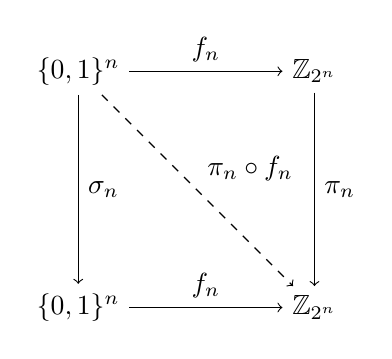
\begin{tikzpicture}[node distance=3cm, auto]
    \node (A) {$\{0,1\}^n$};
    \node (B) [right of=A] {$\mathbb{Z}_{2^n}$};
    \node (C) [below of=A] {$\{0,1\}^n$};
    \node (D) [below of=B] {$\mathbb{Z}_{2^n}$};
    \draw[->] (A) to node {$f_n$} (B);
    \draw[->] (C) to node {$f_n$} (D);
    \draw[->] (A) to node {$\sigma_n$} (C);
    \draw[->] (B) to node {$\pi_n$} (D);
    \draw[->, dashed] (A) to node {$\pi_n \circ f_n$} (D);
\end{tikzpicture}


% \begin{corollary}
% Let $P_\pi$ be the associated permutation matrix to $\pi$. Consider $(c_0, \dots, c_{n-1}) \in \{0,1\}^2$ and its mapping $c \in \mathbb{Z}_{2^n}$. Then 
% \begin{align}
%     P_\pi \ket{c} = \ket{\pi(c)} = \sigma
% \end{align}
% \end{corollary}

\begin{corollary}
All cycles of $\pi_n$ are of order $n$ (except for the all 0s and all 1s strings in which $\pi_n$ acts as the identity).
\end{corollary}
\noindent Proof: Apply lemmas 2 and 5. \qed

(Attempted proof of conjecture 2): Consider a cut $\textbf{c} = (c_0, c_1, c_2, c_3, c_4) \in \{0,1\}^5$. For any $i \in V$ denote its second neighborhood as $\boldsymbol{c_i} = (c_{i-2},c_{i-1},c_i,c_{i+1},c_{i+2})$ with respect to $\textbf{c}$ where the indices are in $\mathbb{Z}_5$. Let $j \in \mathbb{Z}_5$. Then
\begin{align*}
H_j \boldsymbol{c_i} = h(j-1, \boldsymbol{c_i}) + h(j,\boldsymbol{c_i}) + h(j + 1,\boldsymbol{c_i})
\end{align*}

\begin{align*}
    P_{\pi^{-j}} H_0 P_{\pi^j}\boldsymbol{c_i} &=  P_{\pi^{-j}} H_0 \boldsymbol{c_{\pi^{-j}(i)}}\\
    &= P_{\pi^{-j}} (h(-1, \boldsymbol{c_{\pi^{-j}(i)}}) + h(0, \boldsymbol{c_{\pi^{-j}(i)}}) + h(1,\boldsymbol{c_{\pi^{-j}(i)}})) \\
    % &= h(-1, \boldsymbol{c_i}) + h(0, \boldsymbol{c_i}) +
    %  h(1, \boldsymbol{c_i}) \\
     &= h(\pi^{j}(-1), \boldsymbol{c_{\pi^{j}\pi^{-j}(i)}}) + h(\pi^{j}(0), \boldsymbol{c_{\pi^{j}\pi^{-j}(i)}}) +
     h(\pi^{j}(1), \boldsymbol{c_{\pi^{j}\pi^{-j}(i)}})
\end{align*}

\begin{align*}
    P_{\pi^{-j}} H_0 P_{\pi^j}\boldsymbol{c_i} &=  P_{\pi^{-j}} H_0 \boldsymbol{c_{\pi^{-j}(i)}}\\
    &= P_{\pi^{-j}} (h(-1, \boldsymbol{c_{\pi^{-j}(i)}}) + h(0, \boldsymbol{c_{\pi^{-j}(i)}}) + h(1,\boldsymbol{c_{\pi^{-j}(i)}})) \\
    &= h(-1, \boldsymbol{c_i}) + h(0, \boldsymbol{c_i}) +
     h(1, \boldsymbol{c_i}) \\
     &= h(\pi^{j}(-1), \boldsymbol{c_i}) + h(0, \boldsymbol{c_i}) +
     h(1, \boldsymbol{c_i}) &\text{NOT CLEAR ENOUGH}
\end{align*}
TODO FINISH. Need to clean up definitions of $h$ and $H$. \qed

\begin{lemma}
For all $v \in V$, $H_v$ is a real diagonal matrix so they are Hermitian. This also true for their sum $H$.
\end{lemma}
(Proof omitted, necessary?)

\section*{Unitaries}
Given a Hermition operator $H$ on $\mathbb{C}^{2^n}$ and an angle $\gamma \in [0,2 \pi)$, we have the following definition

\begin{equation}
    U_{H, \gamma} = e^{-i \gamma H}
\end{equation}

Consider the operator $X : \mathbb{C} \rightarrow \mathbb{C}$ given by 

\begin{equation}
    X = \begin{bmatrix}
        0 & 1 \\
        1 & 0
    \end{bmatrix}
\end{equation}

\noindent (the quantum NOT gate). We can extend this to an operator on an $n$-dimensional Hilbert space: for each $j \in [n]$, define 

\begin{equation}
    X_j = \left( \bigotimes_{k = 1}^{j - 1} I \right) \bigotimes X \bigotimes \left( \bigotimes_{k = j+1}^{N} I \right)
\end{equation}

\noindent where $I$ is the $2 \times 2$ identity operator. Then $X_j$ is the one qubit operator that acts as a NOT gate on the $j^{th}$ qubit and as the identity on everything else. Letting $d \equiv 2^n$, $X_j$ is a $d \times d$ matrix. Lastly, we consider the sum of all the $X_j$'s:

\begin{equation}
    \overline{X_n} = \sum_{j = 1}^n X_i
\end{equation}

Given an angle $\beta \in [0,\pi)$, we also have the following definition

\begin{equation}
    U_{\beta} = e^{-i\beta \overline{X_n}}
\end{equation}

Recursive definition of $\overline{X_n}$? Need to figure out how to use it for something useful. Preferably, the spectrum.

\noindent Both $U_{H, \gamma}$ and $U_{\beta}$ are unitary since they are the matrix exponential of Hermitian matrices.

\section*{Conjectures}
\begin{conjecture}
For all $j \in \mathbb{Z}_n$, $H_j = P_{\pi^{-j}} H_0 P_{\pi^j}$.
\end{conjecture}
1 is proven for $n=5$. In order to prove higher dimensions, I think it is sufficient to prove the following conjecture.
\begin{conjecture}
Let $H_0 \in M_{2^5}$ be the diagonal matrix whose $i^{th}$ entry is the amount of happy vertices in the second neighborhood of $0$ and let $H_0^n \in M_{2^n}$ be defined similarly for $n \geq 5$. Then
\begin{align*}
    H_0^n = H_0 \otimes \overbrace{I_2 \otimes \cdots \otimes I_2}^{n-1}
\end{align*}
\end{conjecture}

\begin{conjecture}
$\bra{+}U(H, -\gamma) U(-\beta) H U(\beta)U(H, \gamma)\ket{+}$ can be decomposed into a sum of $\bra{+}U(H_0, -\gamma) U(-\beta) H_0 U(\beta)U(H_0, \gamma)\ket{+}$ where $U(H_0, \gamma)$ needs information on the second neighborhood of $H_0$.
\end{conjecture}

\begin{conjecture}
There exists an $\alpha \in [0,2\pi)$ and a $\beta \in [0,\pi)$ such that 
\begin{align*}
    \bra{+}U(H, -\gamma) U(-\beta) H U(\beta)U(H, \gamma)\ket{+} > 0.95
\end{align*}
\end{conjecture}


\end{document}